% THIS IS SIGPROC-SP.TEX - VERSION 3.1
% WORKS WITH V3.2SP OF ACM_PROC_ARTICLE-SP.CLS
% APRIL 2009
%
% It is an example file showing how to use the 'acm_proc_article-sp.cls' V3.2SP
% LaTeX2e document class file for Conference Proceedings submissions.
% ----------------------------------------------------------------------------------------------------------------
% This .tex file (and associated .cls V3.2SP) *DOES NOT* produce:
%       1) The Permission Statement
%       2) The Conference (location) Info information
%       3) The Copyright Line with ACM data
%       4) Page numbering
% ---------------------------------------------------------------------------------------------------------------
% It is an example which *does* use the .bib file (from which the .bbl file
% is produced).
% REMEMBER HOWEVER: After having produced the .bbl file,
% and prior to final submission,
% you need to 'insert'  your .bbl file into your source .tex file so as to provide
% ONE 'self-contained' source file.
%
% Questions regarding SIGS should be sent to
% Adrienne Griscti ---> griscti@acm.org
%
% Questions/suggestions regarding the guidelines, .tex and .cls files, etc. to
% Gerald Murray ---> murray@hq.acm.org
%
% For tracking purposes - this is V3.1SP - APRIL 2009

\documentclass{acm_proc_article-sp}



\usepackage{tabularx}
\graphicspath{ {images/} }
\newdef{theorem}{Izrek}
\newdef{definicija}{Definicija}
\newdef{lema}{Lema}
\begin{document}
	
	\title{Bitcoin napad s prikrivanjem blokov:\\ Analiza in ublažitev napada}
	\subtitle{Povzetek članka}
	%
	% You need the command \numberofauthors to handle the 'placement
	% and alignment' of the authors beneath the title.
	%
	% For aesthetic reasons, we recommend 'three authors at a time'
	% i.e. three 'name/affiliation blocks' be placed beneath the title.
	%
	% NOTE: You are NOT restricted in how many 'rows' of
	% "name/affiliations" may appear. We just ask that you restrict
	% the number of 'columns' to three.
	%
	% Because of the available 'opening page real-estate'
	% we ask you to refrain from putting more than six authors
	% (two rows with three columns) beneath the article title.
	% More than six makes the first-page appear very cluttered indeed.
	%
	% Use the \alignauthor commands to handle the names
	% and affiliations for an 'aesthetic maximum' of six authors.
	% Add names, affiliations, addresses for
	% the seventh etc. author(s) as the argument for the
	% \additionalauthors command.
	% These 'additional authors' will be output/set for you
	% without further effort on your part as the last section in
	% the body of your article BEFORE References or any Appendices.
	
	\numberofauthors{3} %  in this sample file, there are a *total*
	% of EIGHT authors. SIX appear on the 'first-page' (for formatting
	% reasons) and the remaining two appear in the \additionalauthors section.
	%
	\author{
		% You can go ahead and credit any number of authors here,
		% e.g. one 'row of three' or two rows (consisting of one row of three
		% and a second row of one, two or three).
		%
		% The command \alignauthor (no curly braces needed) should
		% precede each author name, affiliation/snail-mail address and
		% e-mail address. Additionally, tag each line of
		% affiliation/address with \affaddr, and tag the
		% e-mail address with \email.
		%
		% 1st. author
		\alignauthor
		Anej Budihna \\
		\affaddr{Univerza v Ljubljani, Fakulteta za računalništvo in informatiko}\\
		% 2nd. author
		\alignauthor
		Luka Golinar\\
		\affaddr{Univerza v Ljubljani, Fakulteta za računalništvo in informatiko}\\
		% 3rd. author
		\alignauthor 
		Matjaž Glumac \\
		\affaddr{Univerza v Ljubljani, Fakulteta za računalništvo in informatiko}\\
		\and  % use '\and' if you need 'another row' of author names
		% 4th. author
	}
	% There's nothing stopping you putting the seventh, eighth, etc.
	% author on the opening page (as the 'third row') but we ask,
	% for aesthetic reasons that you place these 'additional authors'
	% in the \additional authors block, viz.
	
	\date{30 July 1999}
	% Just remember to make sure that the TOTAL number of authors
	% is the number that will appear on the first page PLUS the
	% number that will appear in the \additionalauthors section.
	
	\maketitle
\begin{abstract}

Bitcoin je prva kriptovaluta, ki še danes prevladuje v popularnosti in količini uporabe. V tem članku je obravnavana  varnostna luknja v obstoječi shemi sistema Bitcoin, ki omogoča, izvajanje napadov s prikrivanjem blokov (block witholding attack - BWA). Ta napad se izvaja nad rudarskimi bazeni (mining pool) in ima lahko velike posledice tako za člane bazena kot tudi za celoten Bitcoin sistem. Avtorji so raziskali nekaj posebnih različic tega napada in poskušali ugotoviti dobiček, ki ga pridobi napadalec. Predlagali so tudi nekaj načinov za preprečitev tega napada, ki se razlikujejo obstoječih predlaganih rešitev.
Namesto odkrivanja ali zmanjšanja motivacije za napad so se avtorji odločili za pristop, ki popolnoma izniči zmožnosti izvajanja takšnega napada, s pomočjo kriptografskih in računskih metod.

\end{abstract}
\keywords{Bitcoin rudarjenje, napad z bločnim prikrivanjem, sebičen rudar, rudarske skupine, zavezujoče sheme}

\section{UVOD} \label{sekcija1}

Bitcoin je popularna kriptovaluta, ki jo je prvi predlagal Satoshi Nakamoto leta 2008 \cite{nakamoto}. Vse izvedene transakcije se hranijo v verigi blokov (blockchain). Veriga blokov je javno dostopna in preverljiva knjiga nakazil na kateri temelji celotno omrežje Bitcoin. Veriga zagotavlja, da je mogoče trošiti samo bitcoine, ki so dejansko v lasti plačnika in omogoča preverjanje stanj denarnic. Vsak blok je sestavljen iz več nakazil, nakazilo pa predstavlja prenos bitcoinov iz ene denarnice v drugo. Vsako nakazilo mora biti podpisano s skrivnim ključem, ki ga hrani denarnica. Polek avtentikacije podpis zagotavlja da nakazila, ki so vedno javna, ni mogoče kasneje spreminjati. Informacija o novem nakazilu oziroma transakciji je vedno poslana vsem zainteresiranim članom omrežja.

Zato, da je veriga blokov vredna zaupanja je potrebno vsako transakcijo overiti s potrditvijo omrežja, temu procesu pravimo rudarjenje (mining). Rudarjenje je razpršen sistem doseganja soglasja, ki ga izvajajo člani omrežja. Rudarji nakazila zberejo in jih zapakirajo v bloke, ki morajo zadoščati zelo strogim pravilom šifriranja, ki ji preverja omrežje.  Bloke se overi tako, da se izračuna njihovo hash vrednost, zato da rudar ustreže zahtevam omrežja mora bloku transakcij dodati žeton (nonce). Iskanje te vrednosti predstavlja glavnino dela, ki jo opravlja rudar. Ko rudar najde pravo vrednost objavi dokaz in ga skupaj z blokom doda v verigo. Za najdbo pravega žetona je nagrajen z 25 novo ustvarjenimi bitcoini. Ta nagrada služi kot motivacija za izvajanje overjanja, z regulacijo pravil šifriranja pa se uravnava dotok novih bitcoinov v omrežje. Rudar v blok transakcij vključi transakcijo nagrade v svojo denarnico, kar onemogoča možnost da bi kdo ukradel njegovo opravljeno delo. Pri tem je treba poudariti, da je rudarjenje ''tekmovalna loterija", kar pomeni, da rudarji tekmujejo med seboj, saj nagrado dobi samo tisti, ki prvi reši uganko, in da je izid tekmovanja močno odvisen od sreče.

Ker rudarjenje temelji na metodi grobe sile in je zelo računsko zahtevno opravilo se rudarji pogosto združujejo v rudarske bazene (mining pool). V takšnih bazenih administratorji porazdeljujejo delo tako, da rudarjem pošljejo podpisan blok transakcij z razponom žetonov, ki jih morajo raziskati. Rudarji pa izvajajo izračune in periodično pošiljajo preverjene žetone ter izračunane hash vrednosti, ki predstavljajo delni dokaz o opravljenem delu (partial proof of work). Izračun teh delnih dokazov je veliko lažji od iskanja polnega dokaza, ki zagotavlja nagrado. Vsakič, ko rudar poskuša najti delni dokaz ima možnost najdbe polnega dokaza, ki ga lahko posreduje administratorju. Administrator nato vknjiži blok in pobere nagrado, ki jo nato porazdeli med sodelujoče rudarje. Delež s katerim je nagrajen vsak rudar je odvisen od količine delnih dokazov, ki jih pošlje administratorju med rudarjenjem. Administratorjev podpis v bloku zagotavlja, da noben izmed rudarjev ne more nagrado pobrati zase.

Toda, ko eden izmed članov bazena najde poln dokaz ima tudi opcijo, da dokaza ne posreduje administratorju. Rudar lahko pošilja vse delne dokaze in zakrije polne dokaze, čeprav nagrade ne more zahtevati zase, lahko na ta način od bazena dobiva deleže nagrade na račun drugih članov, kljub temu, da omrežju ne doprinaša nobenih koristi. Takšen napad je poimenovan napad s prikrivanjem blokov(block witholding attack)\cite{analysisofbitcoin},\cite{financialcryptography}. Trenutno je takšen napad nemogoče zaznati ali preprečiti.

\subsection{Napad s prikrivanjem blokov} \label{sekcija2}

Napad s prikrivanjem blokov je bil v prvo predlagan leta 2011 \cite{analysisofbitcoin}, ko so raziskovalci hkrati dokazali, da lahko napadalec na ta način služi tako da zlorablja računsko moč poštenih rudarjev za lasten dobiček. Napadalčev dobiček izvira tudi iz zmanjšanja verjetnosti zmage bazena, ki je žrtev napada. Na ta način se namreč poveča verjetnost, da bo napadalec našel poln dokaz na bloku transakcij s svojim podpisom. Podobno se lahko več članov bazena združi in skupaj napade konkurenčen bazen. Eden izmed največjih takšnih napadov je bil zabeležen junija 2014, zaradi katerega so pošteni člani bazena Eligius zabeležili 300 bitcoinov izgube.

V tem članku so avtorji raziskali podoben scenarij, s tem da so se osredotočili na dve variaciji napada. V prvem primeru so raziskali količino dobička, ki jo ustvari napadalec, ki izvede napad s prikrivanjem blokov (BWH) na izbran bazen in je za napad nagrajen s strani drugega bazena. V drugem primeru je model spremenjen tako, da napadalec porazdeli svojo računsko moč in napade oba bazena. Napadalec lahko celo prejme nagrado s strani obeh dveh bazenov. Takšne napade avtorji poimenujejo ''sponzorirani napad s prikrivanjem blokov". Na ta način napadalec z deležem svojih računskih moči poveča možnost zmage za naročnika napada in zase, če ima dodatna sredstva za rudarjenje.  Ta ranljivost Bitcoin sistema močno vpliva na njegovo delovanje, zato avtorji v članku predlagajo nekaj rešitev, ki so jih sami zasnovali.

\subsection{Pregled področja}
Obstaja že več člankov na to temo. En izmed takih je bil posvečen analizi primera, kjer se dva identična bazena napadata med seboj \cite{minnersdilemma}. Izkazalo se je, da v takem primeru oba bazena zaslužita manj kakor bi če napada ne bi izvedla. V drugem članku so avtorji preverili več scenarijev in dokazali, da ta napad prepričljivo poveča dobiček napadalca \cite{powersplitting}. V prvem članku \cite{minnersdilemma} pa je obravnavan primer, kjer določen bazen pošlje svoje člane, da napade konkurenčen bazen. V tem primeru napadalci delijo svoj dobiček z ostalimi člani bazena.

V tem delu avtorji predstavijo nov napad poimenovan ''sponzorirani napad s prikrivanjem blokov". V tem napadu napadalec poveča možnosti zmage vseh drugih rudarjev in bazenov. Zato lahko vzpostavi dogovor z drugim bazenom kjer je nagrajen za zmanjšanje verjetnosti zmage bazena, ki je tarča napada. Dogovor veli, da je napadalec poplačan sorazmerno z dobičkom, ki ga pomaga ustvariti bazenu s katerim sodeluje. Posebnost tega napada v primerjavi tistimi opisanimi v drugih člankih je ta, da tukaj napadalec deluje samostojno, torej ni član drugih bazenov in ves dobiček obdrži zase.

Motivacija za izdelavo tega članka izvira iz tega povečanega dobička. Članek je razdeljen v dva dela. V prvem avtorji analizirajo dobiček napadalca in analizirajo metode za maksimiranje tega dobička. Pokažejo tudi, da je ob določenih pogojih izvajanje napada bolj dobičkonosno od poštenega rudarjenja. Na koncu avtorji predlagajo še nekaj sprememb in izboljšav trenutnega sistema rudarjenja s katerimi bi popolnoma izkoreninili to ranljivost sistema.

\vfill\eject

\section{ANALIZA NAPADA}

\noindent{\large \bfseries Varnostna shema (Commitment scheme)}
\newline
\indent Varnostno shemo $C$ sestavljajo tri verjetnostni algoritmi, ki se izvedejo v polinomskem času:
\begin{enumerate}
\item $C.Setup()$: Za varnostni parameter k vrne javni parameter $CK$.
\item $C.Commit()$: Sprejme bitni niz $x$ in vrne par $(com, decom)$.
\item $C.Open()$: Sprejme $com$ in $decom$, vrne pa vrednost $x$ ali napako.
\end{enumerate}

Pri obravnavi izbranih primerov sponzoriranih napadov, so avtorji postavili nekaj predpostavk. Predpostavili so, da je v bazenih samo en administrator, ki je zadolžen z koordinacijo in računanjem svojih delnih dokazov o delu. Administrator določi nabor transakcij in druge parametre, člani bazena pa poskušajo ustvariti  delni dokaz o delu glede na te parametre. Administrator določi tudi zahtevnostni nivo delih dokazov, ki mu jih rudarji morajo periodično pošiljati za overjanje. Nivo zahtevnosti delnih dokazov mora bit dovolj nizek, zato da ne preobremeni administratorja. Administrator preverja vse dokaze dokler ne najde ustreznega s katerim lahko zahteva nagrado. Predpostavili so tudi, da je administrator pošten in ga ni mogoče podkupiti.

Napad je opisan na sledeči način. Avtorji enačijo računsko moč celotnega Bitcoin sistema z 1. Obravnavajo dva bazena $P$ in $P'$, z računskimi močmi $p$ in $p'$, ter napadalca $\mathcal{A}$ z računsko močjo $\alpha$. Napadalec porazdeli svojo računsko moč na dva dela, prvi del uporabi za zasebno samostojno rudarjenje, drugi del pa za izvajanje napada na bazen. Napadalec se pridruži bazenu $P$, ki je tarča napada, kjer se pretvarja da je pošten rudar in administratorju periodično pošilja delne dokaze o opravljenem delu. V primeru, da napadalec najde poln dokaz, ta dokaz zadrži in ga ne posreduje bazenu ali Bitcoin sistemu.
Napadalec poln dokaz posreduje bazenu $P'$, ki je konkurent bazenu $P$. Bazen $P'$ ima skrivni dogovor z napadalcem $\mathcal{A}$. Vsakič ko napadalec zadrži poln dokaz mu bazen $P'$ ponudi nagrado. Bazen $P'$ lahko zlahka preveri, če je blok, ki ga je posredoval napadalec pristen, če prevzamemo da $P'$ pozna nabor transakcij v bloku. Ker avtorji predpostavijo, da je $P$ javno dostopen bazen je povsem smiselno, da lahko bazen $P'$ dostopa do teh podatkov. Nagrada, ki jo napadalec dobi od bazena $P'$ je odvisna od pričakovanega dodatnega dobička, ki ga ustvari bazen $P'$. Na ta način napadalec in bazen $P'$ oba imata dodaten dobiček na račun poštenih rudarjev bazena $P$. 


\section{UBLAŽITEV NAPADA} \label{sekcija3}
Napad s prikrivanjem blokov je lahko poguben za vse javno dostopne bazene rudarjev, ki omogočajo včlanitev nezanesljivih rudarjev. V času nastanka članka ni obstajal nobena dobra zaščita pred tem tipom napadov. V sorodnem delu je bila je opisana metoda za odkrivanje takih napadov. Administrator bi ustvaril opravilo za člana bazena, za katero ve da je rešitev poln dokaz o opravljenem delu \cite{analysisofbitcoin}. V primeru, da rudar ne posreduje rešitve se tako ujame v past. Slabost tega pristopa je ta, da od administratorja in poštenih rudarjev zahteva trošenje sredstev, ki bi jih lahko namenili rudarjenju. V drugem sorodnem delu, pa je kot rešitev predlagana dodatna nagrada za rudarja, ki najde poln dokaz \cite{noteonblockattack}.
Avtorji v članku predlagajo enostavno spremembo obstoječe sheme rudarjenja, ki  bi preprečila napad tako s strani članov bazena kot tudi administratorja bazena.


\subsection{Predlagana shema}
V obstoječi shemi je poln dokaz hash vrednost, bloka in žetona, ki ima na najbolj pomembnih bitih $z$ ničel. Delni dokazi o opravljenem delu pa so nizi, ki imajo $z'$ začetnih ničelnih bitov, kjer je $z' < z$.
Delne dokaze rudarji pošiljajo administratorju, ki jih zbira in preverja. Administrator je odgovoren za določitev vrednosti $z'$, ki mora biti taka, da lahko rudarji redno najdejo dokaz in hkrati ne presežejo računskih sposobnosti zaradi preverjanja.
 
Avtorji članka predlagajo sledečo spremembo Bitcoin sheme:
Administrator izbere vrednost $z'$. Bazen poleg tega določi še naključen niz bitov $s$ in vrednost zadnjih $z – z'$ najmanj pomembnih bitov hash vrednosti. Ta niz bitov poimenujemo $r$.
Bazen iz parametrov ustvari varnostno shemo $com$ z ključem $decom$. Administrator pošlje shemo $com$ vsem rudarjem, ključ pa hrani pri sebi in skrbi za to, da ostane tajen. Ko rudarji sestavijo blok vanj vključijo tudi shemo $com$ in dolžino ciljne vrednosti delnega dokaza o opravljenem delu ($z'$). Rudarji administratorju posredujejo vse bloke, ki imajo hash vrednosti z $z'$ začetnimi ničlami. Administrator prejme bloke in med preverjanjem išče takega, ki ustreza začetnim kriterijem. V primeru da najde takšen blok, ga posreduje Bitcoin sistemu skupaj z ključem. Ko vsa vozlišča v sistemu prejmejo blok in ključ, shemo odklenejo in preverijo, če ustreza kriterijem. Blok je sprejet, če je prvih $z$ bitov hash vrednosti sestavljenih iz $z'$ ničel in niza $r$.
 
V tej shemi rudarji ne morejo razlikovati med delnim in polnim dokazom dela. Ko se zamenja obdelovani blok mora administrator razkriti ključ s katerim rudarji preverijo svoje izračunane dokaze. Na ta način rudarjem odvzamemo sposobnost izvajanja dokazov, od administratorja pa zahtevamo dokazovanje poštenosti. Avtorji članka so dokazali, da ta shema ne vpliva na težavnost rudarjenja. Avtorji so predlagali tudi alternativno shemo, kjer kjer se namesto varnostne sheme uporablja hash funkcijo vsi ostali koraki in delovanje pa ostaneta enaka. Obe shemi sta varni dokler sta vrednosti $s$ in $r$ tajni.

\begin{figure}
  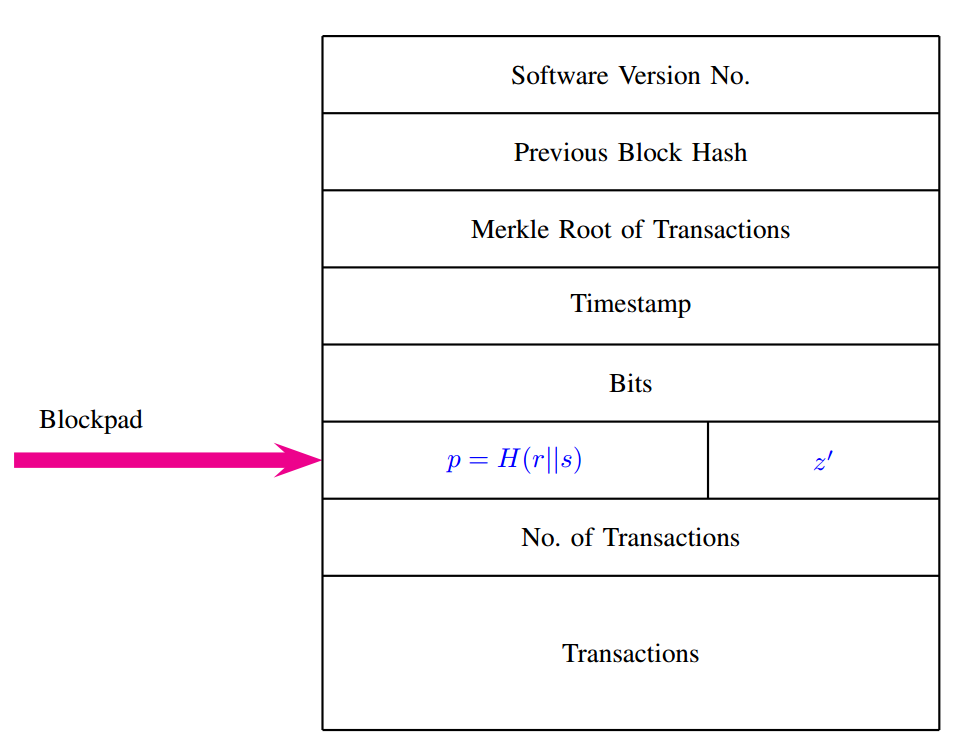
\includegraphics[scale=0.30]{image10.png}
  \caption{Nova shema za rudarjenje}
  \label{fig:boat3}
\end{figure}

\section{ZAKLJUČEK}
Avtorji so v tem članku pokazali kako lahko sebičen rudar pridobi dodaten zaslužek za izvajanje napada s prikrivanjem blokov. Ta dobiček dobi od drugih bazenov, ki si prav tako želijo povečati zaslužek potom tega napada. Izmerili so pričakovan dobiček napadalca in razkrili nekaj zanimivih strategij s katerimi si napadalec lahko poveča dobiček. Predstavili so tudi ukrep s katerimi bi lahko izničili zmožnosti takšnega napada s pomočjo preprostih kriptografskih metod. Ukrep temelji na slepljenju rudarjev in odvzemanju sposobnosti napada ter zavezovanju administratorja v sistem, kjer rudarji lahko preverijo njegovo poštenost. Ukrep je mogoče zlahka implementirati in to brez spreminjanja količine dela, ki je potrebna za izračun delnega dokaza o opravljenem delu.

\newpage
\begin{thebibliography}{9}
 
 \bibitem{nakamoto}
 S. Nakamoto, 
 \textit{Bitcoin: A peer-to-peer electronic cash system}, 2008.
 
 \bibitem{permacoin}
 A. Miller, A. Juels, E. Shi, B. Parno, and J. Katz, 
 \textit{Permacoin: Repurposing bitcoin work for data preservation}, in 2014 IEEE Symposium on Security and Privacy, SP 2014, Berkeley, CA, USA, May 18-21, 2014. IEEE Computer Society, 2014, pp. 475–490.
 
 \bibitem{retriecoin}
 B. Sengupta, S. Bag, S. Ruj, and K. Sakurai, 
 \textit{Retricoin: Bitcoin based on compact proofs of retrievability}, in Proceedings of the 17th International Conference on Distributed Computing and Net- working, ser. ICDCN ’16, 2016, pp. 14:1–14:10.
 
 \bibitem{economicsofbitcoin}
 J. A. Kroll, I. C. Davey, and E. W. Felten, 
 \textit{The economics of bitcoin mining, or bitcoin in the presence of adversaries,}Proceedings of WEIS, vol. 2013, 2013.
 
 \bibitem{analysisofbitcoin}
 M. Rosenfeld,
 \textit{Analysis of bitcoin pooled mining reward systems}, CoRR, vol. abs/1112.4980, 2011. [Online]. Available: http://arxiv.org/abs/1112.4980
 
 \bibitem{financialcryptography}
 A. Laszka, B. Johnson, and J. Grossklags, 
 \textit{Financial Cryptography and Data Security: FC 2015 International Workshops, BITCOIN, WAHC, and Wearable, San Juan, Puerto Rico, January 30, 2015, Revised Selected Papers.} Berlin, Heidelberg: Springer Berlin Heidelberg, 2015, ch. When Bitcoin Mining Pools Run Dry, pp. 63–77.
 
 \bibitem{minnersdilemma}
 . Eyal, 
 \textit{The miner’s dilemma}, in 2015 IEEE Symposium on Security and Privacy, SP 2015, San Jose, CA, USA, May 17-21, 2015. IEEE Computer Society, 2015, pp. 89–103.
 
 \bibitem{powersplitting}
 L. Luu, R. Saha, I. Parameshwaran, P. Saxena, and A. Hobor, 
 \textit{On power splitting games in distributed computation: The case of bit- coin pooled mining}, in IEEE 28th Computer Security Foundations Symposium, CSF 2015, Verona, Italy, 13-17 July, 2015, C. Fournet, M. W. Hicks, and L. Vigano`, Eds. IEEE Computer Society, 2015, pp. 397–411.
 
 \bibitem{subversivestrategies}
 N. T. Courtois and L. Bahack, 
 \textit{On subversive miner strategies and block withholding attack in bitcoin digital currency}, arXiv preprint arXiv:1402.1718, 2014.
 
 \bibitem{datamininglectures}
 I. Damg{\'a}rd, 
 \textit{Lectures on Data Security: Modern Cryptology in The- ory and Practice.} Berlin, Heidelberg: Springer Berlin Heidelberg, 1999, ch. Commitment Schemes and Zero-Knowledge Protocols, pp. 63–86.
 
 \bibitem{incentivecompability}
 D. B. Okke Schrijvers, Joseph Bonneau and T. Roughgarde, 
 \textit{In- centive compatibility of bitcoin mining pool reward functions}, in Financial Cryptography and Data Security: FC 2016 International Workshops.
 
 \bibitem{noteonblockattack}
 S. Bag and K. Sakurai, 
 \textit{Yet another note on block withholding attack on bitcoin mining pools}, in Information Security - 19th International Conference, ISC 2016, Honolulu, HI, USA, September 3-6, 2016, Proceedings, ser. Lecture Notes in Computer Science,
 M. Bishop and A. C. A. Nascimento, Eds., vol. 9866. 2016, pp. 167–180.
 
 \bibitem{originalarticle}
 Samiran Bag, Sushmita Ruj and Kouichi Sakurai,
\textit{Bitcoin Block Withholding Attack : Analysis and
Mitigation}
IEEE Transactions on Information Forensics and Security
\end{thebibliography}
\end{document}

